% Desenvolvido por: Prof. Dr. David Buzatto
%
% Versão 1.0.0
% Data: 22/12/2022
\documentclass[aspectratio=169]{beamer}

\usepackage{estruturaApresentacao}
\usepackage[alf,abnt-emphasize=bf]{abntex2cite}

\begin{document}

\titulo{Título}
% caso não haja, comente a linha abaixo
\subtitulo{subtítulo (se houver)}

\autor{Nome Completo}
\orientador{Prof./Profa. Me./Dr./Dra. Nome Completo}
% caso não haja, comente a linha abaixo
\coorientador{Prof./Profa. Me./Dr./Dra. Nome Completo}

\curso{Nome do Curso}

%exemplos
%\curso{Bacharelado em Ciência da Computação}
%\curso{Tecnologia em Sistemas para Internet}
%\curso{Especialização em Desenvolvimento de Aplicações para Dispositivos Móveis}

\local{São João da Boa Vista}
\dia{DIA}
\mes{MÊS}
\ano{ANO}


\begin{center}
   	
   	\ABNTEXchapterfont\Large\textsc{\imprimirautor}
   	\vspace{2.5cm}
   	
   	\ABNTEXchapterfont\LARGE\textsc{\imprimirtitulo\ifdef{\osubtitulo}{:}{}}

    \ifdef{\osubtitulo}{\ABNTEXchapterfont\Large\imprimirsubtitulo}{}
   	\vspace{2.5cm}
   	   	
   	\hspace{.4\textwidth}
   	\begin{minipage}{.5\textwidth}
   		\SingleSpacing
   		\large\imprimirpreambulo
   		
   		\vspace{\onelineskip}
   		
   		Orientador: \imprimirorientador
   		
        \ifdef{\ocoorientador}{
            \vspace{\onelineskip}
               		
       		Coorientador: \imprimircoorientador
        }{}
        
        
   		
   	\end{minipage}%
    \vfill
   	
   	\Large\textsc{\imprimirlocal}
   	
   	\Large\textsc{\imprimirano}
   	
   	\vspace*{2cm}
   	
\end{center}
\section{Introdução}

\begin{frame}

    \frametitle{Introdução}

    Apresente a introdução do seu trabalho.

\end{frame}


\begin{frame}

    \frametitle{Objetivos}

    \begin{itemize}
    
        \item Objetivo Geral
            \begin{itemize}
                \item Objetivo geral do trabalho.
            \end{itemize}
            
        \item Objetivos Específicos
            \begin{itemize}
                \item Objetivo específico 1;
                \item Objetivo específico 2;
                \item ...;
                \item Objetivo específico n.
            \end{itemize}
            
    \end{itemize}

\end{frame}
\section{Revisão da Literatura/Considerações Gerais}


\subsection{Assunto 1}

\begin{frame}

    \frametitle{Assunto 1}

    Slide 1 assunto 1...

\end{frame}


\begin{frame}

    \frametitle{Assunto 1}

    Slide 2 do assunto 1...

\end{frame}


\subsection{Assunto 2}

\begin{frame}

    \frametitle{Assunto 2}

    Slide 1 do assunto 2...

\end{frame}


\begin{frame}

    \frametitle{Assunto 2}

    Slide 2 do assunto 2...

\end{frame}


\subsection{Assunto n}

\begin{frame}

    \frametitle{Assunto n}

    Slide 1 do assunto n...

\end{frame}


\begin{frame}

    \frametitle{Assunto n}

    Slide 2 do assunto n...

\end{frame}
\section{Metodologia}


\begin{frame}

    \frametitle{Metodologia}

    Slide 1 da metodologia...
    
    Sugestão: utilize um diagrama para apresentar de forma geral sua metodologia.

\end{frame}


\begin{frame}

    \frametitle{Metodologia}

    Slide 2 da metodologia...

\end{frame}


\begin{frame}

    \frametitle{Metodologia}

    Slide n da metodologia...

\end{frame}
\section{Resultados}


\begin{frame}

    \frametitle{Resultados}

    Slide 1 dos resultados...

\end{frame}


\begin{frame}

    \frametitle{Resultados}

    Slide 2 dos resultados...

\end{frame}


\begin{frame}

    \frametitle{Resultados}

    Slide n dos resultados...

\end{frame}
\section{Conclusão e Trabalhos Futuros}


\begin{frame}

    \frametitle{Conclusão e Trabalhos Futuros}

    Slide 1 da conclusão...

\end{frame}


\begin{frame}

    \frametitle{Conclusão e Trabalhos Futuros}

    Slide 2 da conclusão...

\end{frame}


\begin{frame}

    \frametitle{Conclusão e Trabalhos Futuros}

    Slide n da conclusão...

\end{frame}


\begin{frame}
    \begin{center}
        \Huge{OBRIGADO!}
    \end{center}
\end{frame}


% exemplos de construções em LaTeX
% comente a linha abaixo para gerar a versão final
\section{Exemplos}


\begin{frame}

    \frametitle{Título do Slide}

    Texto corrido normal .
    
    \begin{huge}
        Texto com fonte gigante.
    \end{huge}
    
    \begin{LARGE}
        Texto com fonte GRANDE.
    \end{LARGE}
        
    \begin{Large}
        Texto com fonte Grande.
    \end{Large}
    
    \begin{large}
        Texto com fonte grande.
    \end{large}
    
    \begin{normalsize}
        Texto com fonte normal.
    \end{normalsize}
        
    \begin{small}
        Texto com fonte pequena.
    \end{small}
        
    \begin{footnotesize}
        Texto com fonte do tamanho de nota de rosapé.
    \end{footnotesize}
    
    \begin{scriptsize}
        Texto com fonte do tamanho de letra manuscrita.
    \end{scriptsize}
        
    \begin{tiny}
        Texto com fonte minúscula.
    \end{tiny}        

\end{frame}


\begin{frame}

    \frametitle{Slide com Duas Colunas}
    
    \begin{columns}[t]
    
        \begin{column}{7cm}

            Conteúdo da coluna 1.

        \end{column}

        \begin{column}{7cm}

            Conteúdo da coluna 2.

        \end{column}

    \end{columns}
        
\end{frame}


\begin{frame}

    \frametitle{Slide com Blocos}
    
    Exemplos de blocos de texto. Cuidado para não abusar no uso, evitando que os slides fiquem muito ``carregados''.
    
    \begin{block}{Observação}
        Caixa de texto padrão.
    \end{block}
    
    \begin{exampleblock}{Exemplo}
        Caixa de texto de exemplo.
    \end{exampleblock}
        
    \begin{alertblock}{Importante}
        Caixa de texto de alerta.
    \end{alertblock}
    
    \definecolor{corFundoTitulo}{RGB}{95, 40, 113}
    \definecolor{corTextoTitulo}{RGB}{255, 255, 255}
    \definecolor{corFundoConteudo}{RGB}{114, 140, 166}
    \definecolor{corTextoConteudo}{RGB}{0, 0, 0}
    \begin{bloco}{Bloco com cores customizadas}{bg=corFundoConteudo,fg=corTextoConteudo}{bg=corFundoTitulo,fg=corTextoTitulo}
        Conteúdo
    \end{bloco}
         
\end{frame}


\begin{frame}

    \frametitle{Slide com Desenhos Usando Tikz}
    
    Desenhando formas...
    
    \begin{center}
        
\begin{tikzpicture}[scale=1.0]
            \draw[blue, very thick] (0,0) rectangle (3,2);
            \draw[orange, ultra thick] (4,0) -- (6,0) -- (5.7,2) -- cycle;
        \end{tikzpicture}
    \end{center}
         
\end{frame}


\begin{frame}

    \frametitle{Slide com Desenhos Usando Tikz}
    
    Uma Máquina de Turing que realiza a operação subtração própria.
    
    \begin{center}
        \begin{tikzpicture} [scale=0.75, every node/.style={transform shape}, node distance = 3cm, on grid]

            \node (q0) [state,
                initial,
                initial text=Início
            ] {$q_0$};
            \node (q1) [state, right = of q0] {$q_1$};
            \node (q2) [state, right = of q1] {$q_2$};
            \node (q3) [state, right = of q2] {$q_3$};
            \node (q5) [state, below = of q0] {$q_5$};
            \node (q6) [state, below = of q1] {$q_6$};
            \node (q4) [state, below = of q2] {$q_4$};
                        
            \path [-stealth]
                (q0) edge node[above] {$0/B\rightarrow$} (q1)
                (q1) edge [loop below] node {$0/0\rightarrow$} ()
                (q1) edge node[above] {$1/1\rightarrow$} (q2)
                (q2) edge [loop below] node[right] {$1/1\rightarrow$} ()
                (q2) edge node[above] {$0/1\leftarrow$} (q3)
                
                (q3) edge [loop below] node {$
                    \begin{aligned}
                      0 &/ 0\leftarrow\\[-0.7ex]
                      1 &/ 1\leftarrow
                    \end{aligned}$} ()
                
                (q3) edge [bend right] node[above] {$B/B\rightarrow$} (q0)
                
                (q0) edge [bend right] node[left] {$1/B\rightarrow$} (q5)
                (q2) edge [bend right] node[left] {$B/B\leftarrow$} (q4)
                
                (q5) edge [loop below] node {$
                    \begin{aligned}
                      0 &/ B\rightarrow\\[-0.7ex]
                      1 &/ B\rightarrow
                    \end{aligned}$} ()
                                    
                (q5) edge node[above] {$B/B\rightarrow$} (q6)
                
                (q4) edge [loop below] node {$
                    \begin{aligned}
                      0 &/ 0\leftarrow\\[-0.7ex]
                      1 &/ B\leftarrow
                    \end{aligned}$} ()
                                    
                (q4) edge node[above] {$B/0\rightarrow$} (q6);
        
        \end{tikzpicture}
    \end{center}
         
\end{frame}


\begin{frame}

    \frametitle{Slide com Figura}
    
    \begin{figure}[!htbp]
       	\centering
       	\caption{Exemplo de figura (caption é opcional)}
       	
\includegraphics[scale=0.3]{imagens/exemploFigura}
        \\\small{\textbf{Fonte:} Elaborada pelo autor (fonte é opcional)}%
     \end{figure}
         
\end{frame}


\begin{frame}

    \frametitle{Slide com Tabela}
    
    \begin{table}[!htbp]
       	\centering
       	\caption{Exemplo de tabela de 2 colunas (caption é opcional)}
       	\begin{tabular}{ c | c }
       		\hline
       		\textbf{Coluna 1} & \textbf{Coluna 2} \\ \hline
       		Dado 1a           & Dado 2a           \\ \hline
       		Dado 1b           & Dado 2b           \\ \hline
       		Dado 1c           & Dado 2c           \\ \hline
       		Dado 1d           & Dado 2d           \\ \hline
       	\end{tabular}
       	\\ \vspace{0.2cm}
       	\small{\textbf{Fonte:} Elaborada pelo autor (fonte é opcional)}%
     \end{table}
         
\end{frame}


\begin{frame}

    \frametitle{Slide com Quadro}
    
    \begin{quadro}[!htbp]
       	\centering
       	\caption{Exemplo de quadro (caption é opcional)}
       	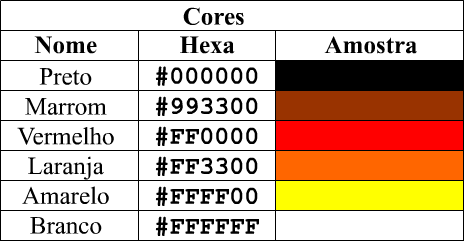
\includegraphics[scale=.3]{imagens/exemploQuadro}
        \\ \vspace{0.2cm}
       	\small{\textbf{Fonte:} Elaborada pelo autor (fonte é opcional)}%
    \end{quadro}
         
\end{frame}


\begin{frame}

    \frametitle{Slide com Equação}
    
    \begin{equation}
        \sum_{i=1}^{n} i = \frac{n(n+1)}{2}
        \label{eq:exemplo}
    \end{equation}
         
\end{frame}


\begin{frame}

    \frametitle{Slide com Código Fonte}
    
    \centering
    \resizebox{10cm}{!}{%
        \lstinputlisting[language=Java]{fontes/ClasseExemplo.java} 
    }
    
\end{frame}


\begin{frame}

    \frametitle{Slide com Lista de Itens}
    
    \begin{itemize}
       	\item \textbf{Item 1:} texto...;
       	\item \textbf{Item 2:} texto...;
       	\begin{itemize}
       		\item \textbf{Subitem:} texto...;
       		\item \textbf{Subitem:} texto...;
       		\item \textbf{Subitem:} texto...;
       	\end{itemize}
       	\item \textbf{Item 3:} texto...;
       	\item \textbf{Item n:} texto....
    \end{itemize}
         
\end{frame}


\begin{frame}

    \frametitle{Slide com Lista Numerada}
    
    \begin{enumerate}
       	\item \textbf{Item:} texto...;
       	\item \textbf{Item:} texto...;
       	\begin{enumerate}
       		\item \textbf{Subitem:} texto...;
       		\item \textbf{Subitem:} texto...;
       		\item \textbf{Subitem:} texto...;
       	\end{enumerate}
       	\item \textbf{Item:} texto...;
       	\item \textbf{Item:} texto....
    \end{enumerate}
         
\end{frame}


\begin{frame}

    \frametitle{Formatação de Texto e Referências}
    
    Todas as macros que você utilizou na elaboração do seu documento podem ser usadas nas apresentações, com exceção do ambiente verbatim. Você poderá criar citações formatadas também, mas as referências não serão geradas em um slide, apenas serão exibidas no texto. Por exemplo:
    
    \begin{itemize}
        \item \cite{Abedi2014, Agaisse1995};
        \item \cite{AgapitoTenfen2014, BtNomenclature2016, Nelson2014};
        \item \citeauthorandyear{Agaisse1995};
        \item \citeauthorandyear{Abedi2014};
        \item \citeauthorandyear{BtNomenclature2016};
    \end{itemize}
         
\end{frame}


% não mexa!

\begin{frame}<presentation:0>
    \addtocounter{framenumber}{-1}
    \bibliography{referencias}
\end{frame}

\end{document} 